\documentclass[11pt]{beamer}
\usetheme{Boadilla}
\usefonttheme{serif}
% \setbeamertemplate{navigation symbols}{}

\usepackage[T1]{fontenc}
\usepackage[utf8]{inputenc}
\usepackage{lmodern}
\usepackage{booktabs}
\usepackage{graphicx}
\usepackage{adjustbox}
\usepackage{xcolor}
\usepackage{amsmath}
\usepackage{tikz}
\usepackage{hyperref}

% \definecolor{imfblue}{RGB}{0,78,130}
\definecolor{darkred}{RGB}{170,20,30}
% \setbeamercolor{structure}{fg=imfblue}
% \setbeamercolor{title}{fg=imfblue}
% \setbeamercolor{frametitle}{fg=imfblue}
\setbeamercolor{alerted text}{fg=darkred}
% \setbeamertemplate{itemize item}{\color{imfblue}$\blacktriangleright$}
% \setbeamertemplate{itemize subitem}{\color{imfblue}$\circ$}

\newcommand{\widefig}[2]{\begin{center}\includegraphics[#1]{#2}\end{center}}
\newcommand{\slideclaim}[1]{\vspace{-0.1cm}{#1}}
\newcommand{\hit}[1]{\fcolorbox{darkred}{white}{\strut #1}}

\title[Changing Global Linkages]{Changing Global Linkages: A New Cold War?}
\subtitle{Gita Gopinath et al., \textit{Journal of International Economics}, 153, 2025.}
\author{Jingle Fu}
\date{\today}

\begin{document}

\begin{frame}
  \titlepage
\end{frame}

% \begin{frame}{Argument in one sentence}
%   Globalization has not collapsed in aggregate, but bilateral trade, FDI, and portfolio positions increasingly sort along geopolitical lines after 2022, while nonaligned connector economies partly preserve indirect links between rival blocs.
%   \begin{enumerate}
%     \item The empirical object is the \alert{direction} of flows, not only global trade to GDP.
%     \item The paper uses reallocation indices, gravity estimates, and a Cold War benchmark.
%     \item The main mechanism is not simple reshoring, but rerouting through connector economies.
%     \item The critique should focus on method choices, omitted margins, and economic interpretation.
%   \end{enumerate}
% \end{frame}

% \begin{frame}{Presentation structure}
%   \begin{enumerate}
%     \item Motivation: why aggregate globalization misses bilateral fragmentation.
%     \item Measurement: blocs, nonaligned countries, and the Modified Lilien Index.
%     \item Main estimates: Table 1 and the gravity interpretation.
%     \item Dynamics: current fragmentation versus the early Cold War.
%     \item Connector countries: why today's world differs from the 1950s.
%     \item Critical assessment: method choices, omitted margins, and scope limits.
%   \end{enumerate}
% \end{frame}

\begin{frame}{Introduction}
  \widefig{height=0.62\textheight}{replication_audit/charts_original/F1L.png}
  \vspace{-0.2cm}
  \slideclaim{Aggregate trade has not collapsed. Fragmentation can occur beneath a high and stable global trade to GDP ratio. The Cold War is the historical case where global openness rose while East West trade remained politically constrained.}
\end{frame}

\begin{frame}{Introduction}
  \widefig{height=0.60\textheight}{replication_audit/charts_original/F1R.png}
  \slideclaim{Trade growth falls more between geopolitical blocs than within blocs after the Ukraine war. The relevant outcome is the relative performance of politically distant links, not aggregate trade growth alone.}
\end{frame}

\begin{frame}{Key Questions}
  \begin{itemize}
    \item Is fragmentation the reality?
    \item How serious is the fragmentation compare to the Cold War?
    \item What is the role of nonaligned countries?
  \end{itemize}
\end{frame}

\begin{frame}{Introduction}
  \widefig{width=\textwidth}{replication_audit/charts_original/FS1.1.png}
\end{frame}

\begin{frame}{Data}
  \begin{tabular}{p{0.2\textwidth}p{0.32\textwidth}p{0.36\textwidth}}
    \toprule
    Object                & Source                                    & Role in the argument                                   \\
    \midrule
    Goods trade           & Trade Data Monitor, TRADHIST, CEPII       & Current bilateral trade and Cold War comparison        \\
    FDI                   & fDi Markets announced greenfield projects & Investment sorting, mainly using project counts        \\
    Portfolio             & IMF CPIS bilateral holdings               & Financial sorting through portfolio shares             \\
    Geopolitical distance & UN voting ideal point distance            & Define within bloc, between bloc, and nonaligned pairs \\
    \bottomrule
  \end{tabular}
\end{frame}

\begin{frame}{Bloc classification}
  \begin{itemize}
    \item Wider definition: countries are assigned using ideal point distance from the United States and China.
    \item Narrower definition:
          \begin{itemize}
            \item West Bloc: United States, Europe, Canada, Australia, and New Zealand;
            \item East Bloc: Belarus, China, Eritrea, Mali, Nicaragua, Russia, and Syria.
          \end{itemize}
          % \item Nonaligned countries are not a residual nuisance. They are central because they may act as bridges.
          % \item This is why the paper checks wider and narrower bloc definitions throughout the main table.
  \end{itemize}
  \slideclaim{The estimates are conditional on a political map. The wider definition uses continuous geopolitical distance, while the narrow definition asks whether the result survives a more conservative bloc assignment.}
\end{frame}

\begin{frame}{Reallocation: The Modified Lilien Index}
  \[
    MLI_{rt} =
    \sqrt{\sum_i S_{irt}
      \left[
        \left( \ln x_{irt} / \ln x_{irt-1} \right)  - \left( \ln X_{rt} / X_{rt-1} \right)
        \right]^2}
  \]
  \begin{itemize}
    \item $x_{irt}$ is imports or FDI from partner $i$ into country $r$.
    \item $X_{rt}$ is total imports or FDI of country $r$.
    \item $S_{irt}$ is the share of trade or FDI from partner $i$ to country $r$.
    \item The index is zero if all partners grow at the same rate as total imports or FDI.
  \end{itemize}
\end{frame}

\begin{frame}{Reallocation across import and FDI sources rises after 2022}
  \widefig{height=0.62\textheight}{replication_audit/charts_original/F2L.png}
  \slideclaim{The import source Modified Lilien Index rises sharply in the post 2022 period, especially for advanced economies. The paper treats this as the first sign that firms and countries are changing sourcing partners.}
\end{frame}

\begin{frame}{FDI source reallocation shows the same timing}
  \widefig{height=0.62\textheight}{replication_audit/charts_original/F2R.png}
  \slideclaim{FDI project sourcing also becomes more dispersed after 2022. This matters because investment decisions are forward looking and indicate expected changes in production geography.}
\end{frame}

\begin{frame}{Reallocation across Economies}
  \widefig{height=0.9\textheight}{replication_audit/tables_original/table S2-1.png}
\end{frame}

\begin{frame}{Fragmentation: Gravity model}
  \[
    \begin{array}{rcl}
      Y_{sdt} & = &
      \beta_1 (\text{Between Blocs}_{sd}\times \text{Post}_t)
      + \beta_2 (\text{Nonaligned}_{sd}\times \text{Post}_t) \\
              &   & + \delta_{sd} + \tau_{st} + \phi_{dt}
      + \varepsilon_{sdt}
    \end{array}
  \]
  \vspace{-0.2cm}
  \begin{itemize}
    \item $Y_{sdt}$: cross-border flows from origin $s$ to destination $d$ at time $t$, such as bilateral trade value or FDI amount.
    \item $\text{Between Blocs}_{sd}$: dummy, 1 if origin $s$ and destination $d$ belong to opposing geopolitical blocs, such as the U.S.--Europe bloc vs. the China--Russia bloc.
    \item $\text{Nonaligned}_{sd}$: dummy, 1 if origin $s$ or destination $d$ belongs to a non-aligned country, such as Vietnam or Mexico.
    \item $\text{Post}_{t}$: $\text{Post}_{t}=1$ after the Russia--Ukraine conflict in 2022, 0 for period before.
  \end{itemize}
\end{frame}

\begin{frame}{Table 1, Panel A: wider bloc, trade and FDI}
  \begin{center}
    \begin{adjustbox}{max width=\textwidth}
      \begin{tabular}{lcccc}
        \toprule
                                       & \multicolumn{2}{c}{Trade} & \multicolumn{2}{c}{FDI}                               \\
                                       & (1)                       & (2)                     & (3)        & (4)            \\
        \midrule
        Between Bloc $\times$ Post War & -0.1059**                 & \hit{-0.1212**}         & -0.3614*** & \hit{-0.1309*} \\
                                       & (0.041)                   & (0.058)                 & (0.071)    & (0.074)        \\
        Nonaligned $\times$ Post War   & 0.0403                    & 0.0043                  & -0.0025    & -0.0942        \\
                                       & (0.030)                   & (0.051)                 & (0.046)    & (0.077)        \\
        Observations                   & 259,840                   & 259,780                 & 170,412    & 152,088        \\
        Country-pair FE                & Y                         & Y                       & Y          & Y              \\
        Time FE                        & Y                         & --                      & Y          & --             \\
        Source $\times$ Time FE        & N                         & Y                       & N          & Y              \\
        Destination $\times$ Time FE   & N                         & Y                       & N          & Y              \\
        \bottomrule
      \end{tabular}
    \end{adjustbox}
  \end{center}
  \slideclaim{Under the wider bloc definition, trade and FDI between rival blocs fall relative to within bloc flows. Nonaligned pairs do not show the same pattern.}
\end{frame}

\begin{frame}{Table 1, Panel A: wider bloc, portfolio}
  \begin{center}
    \begin{adjustbox}{max width=\textwidth}
      \begin{tabular}{lcc}
        \toprule
                                       & \multicolumn{2}{c}{Portfolio}                  \\
                                       & (5)                           & (6)            \\
        \midrule
        Between Bloc $\times$ Post War & -0.0417*                      & \hit{-0.0540*} \\
                                       & (0.025)                       & (0.028)        \\
        Nonaligned $\times$ Post War   & -0.0212                       & -0.0363        \\
                                       & (0.021)                       & (0.031)        \\
        Observations                   & 235,093                       & 235,059        \\
        Country-pair FE                & Y                             & Y              \\
        Time FE                        & Y                             & --             \\
        Source $\times$ Time FE        & N                             & Y              \\
        Destination $\times$ Time FE   & N                             & Y              \\
        \bottomrule
      \end{tabular}
    \end{adjustbox}
  \end{center}
  \slideclaim{Portfolio holdings also sort away from cross bloc pairs, supporting the paper's claim that fragmentation is not limited to goods markets.}
\end{frame}

\begin{frame}{Table 1, Panel A: wider bloc, Cold War benchmark}
  \begin{center}
    \begin{adjustbox}{max width=\textwidth}
      \begin{tabular}{lcc}
        \toprule
                                       & \multicolumn{2}{c}{Cold War trade}                    \\
                                       & (7)                                & (8)              \\
        \midrule
        Between Bloc $\times$ Post War & -0.6092***                         & \hit{-1.1076***} \\
                                       & (0.163)                            & (0.110)          \\
        Nonaligned $\times$ Post War   & -0.2612**                          & \hit{-0.4641**}  \\
                                       & (0.110)                            & (0.235)          \\
        Observations                   & 766,007                            & 687,736          \\
        Country-pair FE                & Y                                  & Y                \\
        Time FE                        & Y                                  & --               \\
        Source $\times$ Time FE        & N                                  & Y                \\
        Destination $\times$ Time FE   & N                                  & Y                \\
        \bottomrule
      \end{tabular}
    \end{adjustbox}
  \end{center}
\end{frame}

\begin{frame}{Main Result}
  \begin{itemize}
    \item For PPML trade and FDI estimates, convert coefficients using $\exp(\beta)-1$.
    \item Trade: $\exp(-0.1212)-1=-11.4\%$.
    \item FDI projects: $\exp(-0.1309)-1=-12.3\%$.
    \item Portfolio holdings: the preferred coefficient implies about 0.5 percentage point lower cross bloc portfolio shares relative to within bloc holdings.
    \item The Cold War benchmark is around -67 percent for between bloc trade in the saturated model.
  \end{itemize}
  \slideclaim{The result is moderate in size today, but broad across goods, investment, and financial portfolios.}
\end{frame}

\begin{frame}{Table 1, Panel B: narrower bloc, trade and FDI}
  \begin{center}
    \begin{adjustbox}{max width=\textwidth}
      \begin{tabular}{lcccc}
        \toprule
                                       & \multicolumn{2}{c}{Trade} & \multicolumn{2}{c}{FDI}                                \\
                                       & (1)                       & (2)                     & (3)        & (4)             \\
        \midrule
        Between Bloc $\times$ Post War & -0.1562***                & -0.1194                 & -0.6869*** & \hit{-0.2697**} \\
                                       & (0.053)                   & (0.089)                 & (0.114)    & (0.137)         \\
        Nonaligned $\times$ Post War   & 0.0207                    & 0.0762                  & 0.0129     & 0.1049          \\
                                       & (0.031)                   & (0.077)                 & (0.041)    & (0.071)         \\
        Observations                   & 284,765                   & 284,706                 & 178,464    & 159,388         \\
        Country-pair FE                & Y                         & Y                       & Y          & Y               \\
        Time FE                        & Y                         & --                      & Y          & --              \\
        Source $\times$ Time FE        & N                         & Y                       & N          & Y               \\
        Destination $\times$ Time FE   & N                         & Y                       & N          & Y               \\
        \bottomrule
      \end{tabular}
    \end{adjustbox}
  \end{center}
  \slideclaim{The narrower classification is more conservative. The FDI shortfall remains clear, while trade becomes less precise once country time shocks are absorbed.}
\end{frame}

\begin{frame}{Table 1, Panel B: narrower bloc, portfolio}
  \begin{center}
    \begin{adjustbox}{max width=\textwidth}
      \begin{tabular}{lcc}
        \toprule
                                       & \multicolumn{2}{c}{Portfolio}                  \\
                                       & (5)                           & (6)            \\
        \midrule
        Between Bloc $\times$ Post War & -0.1841**                     & \hit{-0.1763*} \\
                                       & (0.078)                       & (0.101)        \\
        Nonaligned $\times$ Post War   & -0.0146                       & -0.0366        \\
                                       & (0.034)                       & (0.042)        \\
        Observations                   & 260,491                       & 260,457        \\
        Country-pair FE                & Y                             & Y              \\
        Time FE                        & Y                             & --             \\
        Source $\times$ Time FE        & N                             & Y              \\
        Destination $\times$ Time FE   & N                             & Y              \\
        \bottomrule
      \end{tabular}
    \end{adjustbox}
  \end{center}
  \slideclaim{The portfolio estimates remain negative under the narrower bloc definition. This supports the paper's claim that fragmentation is not limited to goods markets.}
\end{frame}

\begin{frame}{Robustness}
  \widefig{height=0.8\textheight}{replication_audit/tables_original/table S2-2.png}
\end{frame}

\begin{frame}{Robustness}
  \widefig{height=0.8\textheight}{replication_audit/tables_original/table S2-3.png}
\end{frame}

\begin{frame}{Recall: Cold War benchmark}
  \begin{center}
    \begin{adjustbox}{max width=\textwidth}
      \begin{tabular}{lcc}
        \toprule
                                       & \multicolumn{2}{c}{Cold War trade}                    \\
                                       & (7)                                & (8)              \\
        \midrule
        Between Bloc $\times$ Post War & -0.6092***                         & \hit{-1.1076***} \\
                                       & (0.163)                            & (0.110)          \\
        Nonaligned $\times$ Post War   & -0.2612**                          & \hit{-0.4641**}  \\
                                       & (0.110)                            & (0.235)          \\
        Observations                   & 766,007                            & 687,736          \\
        Country-pair FE                & Y                                  & Y                \\
        Time FE                        & Y                                  & --               \\
        Source $\times$ Time FE        & N                                  & Y                \\
        Destination $\times$ Time FE   & N                                  & Y                \\
        \bottomrule
      \end{tabular}
    \end{adjustbox}
  \end{center}
\end{frame}

\begin{frame}{Dynamics: current episode versus the Cold War}
  \widefig{height=0.62\textheight}{replication_audit/charts_original/F3A.png}
  \slideclaim{The current red line turns negative after the Ukraine war, but the Cold War blue line becomes far more negative over a longer horizon. The comparison implies early fragmentation rather than completed decoupling.}
\end{frame}

\begin{frame}{Nonaligned economies behave differently today}
  \widefig{height=0.62\textheight}{replication_audit/charts_original/F3B.png}
  \slideclaim{During the Cold War, nonaligned trade also weakened substantially. In the current period, nonaligned trade does not show the same broad collapse, which makes nonaligned countries central rather than peripheral.}
\end{frame}

\begin{frame}{Timing of trade fragmentation}
  % \begin{center}
  %   \begin{minipage}{0.46\textwidth}
  %     \centering
  %     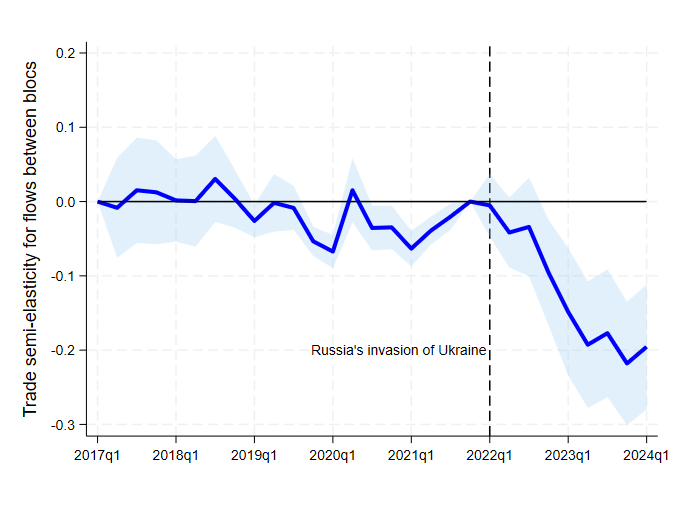
\includegraphics[height=0.35\textheight]{replication_audit/charts_original/FS1.2A.png}\\[-0.15cm]
  %     {\tiny (a) Trade between blocs, now}
  %   \end{minipage}
  %   \hspace{0.035\textwidth}
  %   \begin{minipage}{0.46\textwidth}
  %     \centering
  %     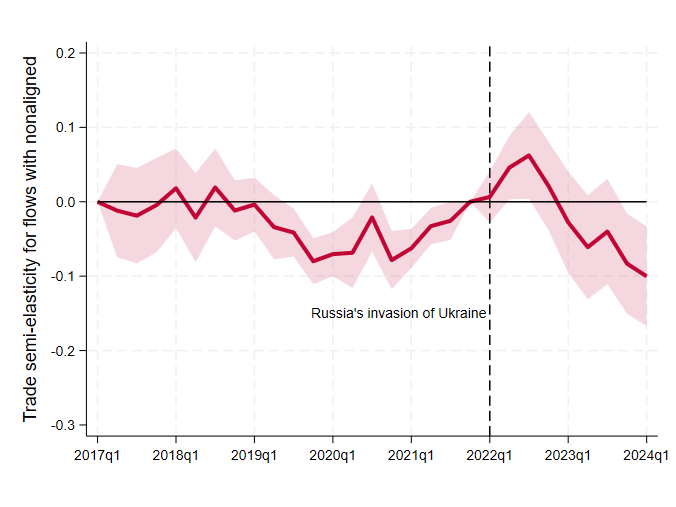
\includegraphics[height=0.35\textheight]{replication_audit/charts_original/FS1.2B.png}\\[-0.15cm]
  %     {\tiny (b) Trade with nonaligned, now}
  %   \end{minipage}

  %   \vspace{-0.12cm}

  %   \begin{minipage}{0.46\textwidth}
  %     \centering
  %     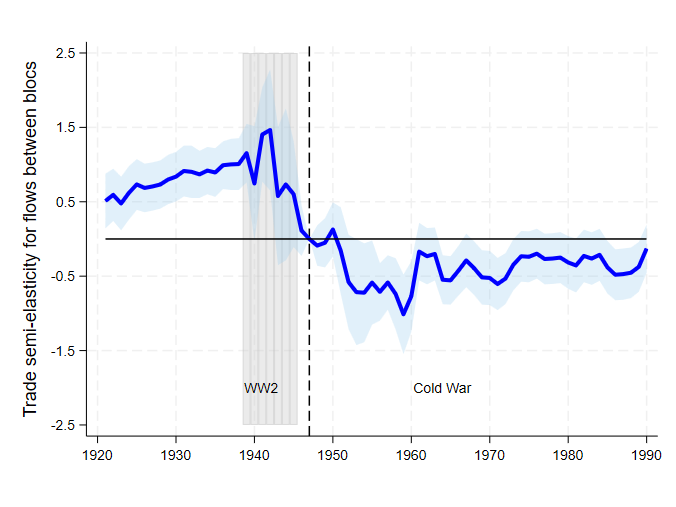
\includegraphics[height=0.35\textheight]{replication_audit/charts_original/FS1.2C.png}\\[-0.15cm]
  %     {\tiny (c) Trade between blocs, Cold War}
  %   \end{minipage}
  %   \hspace{0.035\textwidth}
  %   \begin{minipage}{0.46\textwidth}
  %     \centering
  %     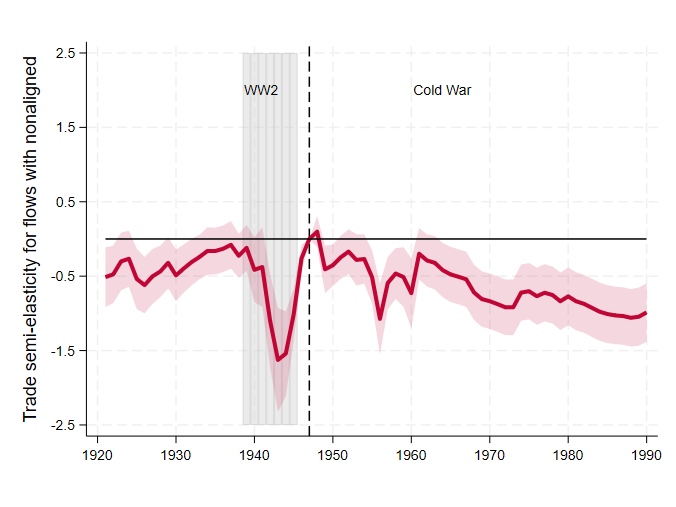
\includegraphics[height=0.35\textheight]{replication_audit/charts_original/FS1.2D.png}\\[-0.15cm]
  %     {\tiny (d) Trade with nonaligned, Cold War}
  %   \end{minipage}
  % \end{center}
  % \vspace{-0.08cm}
  \begin{center}
    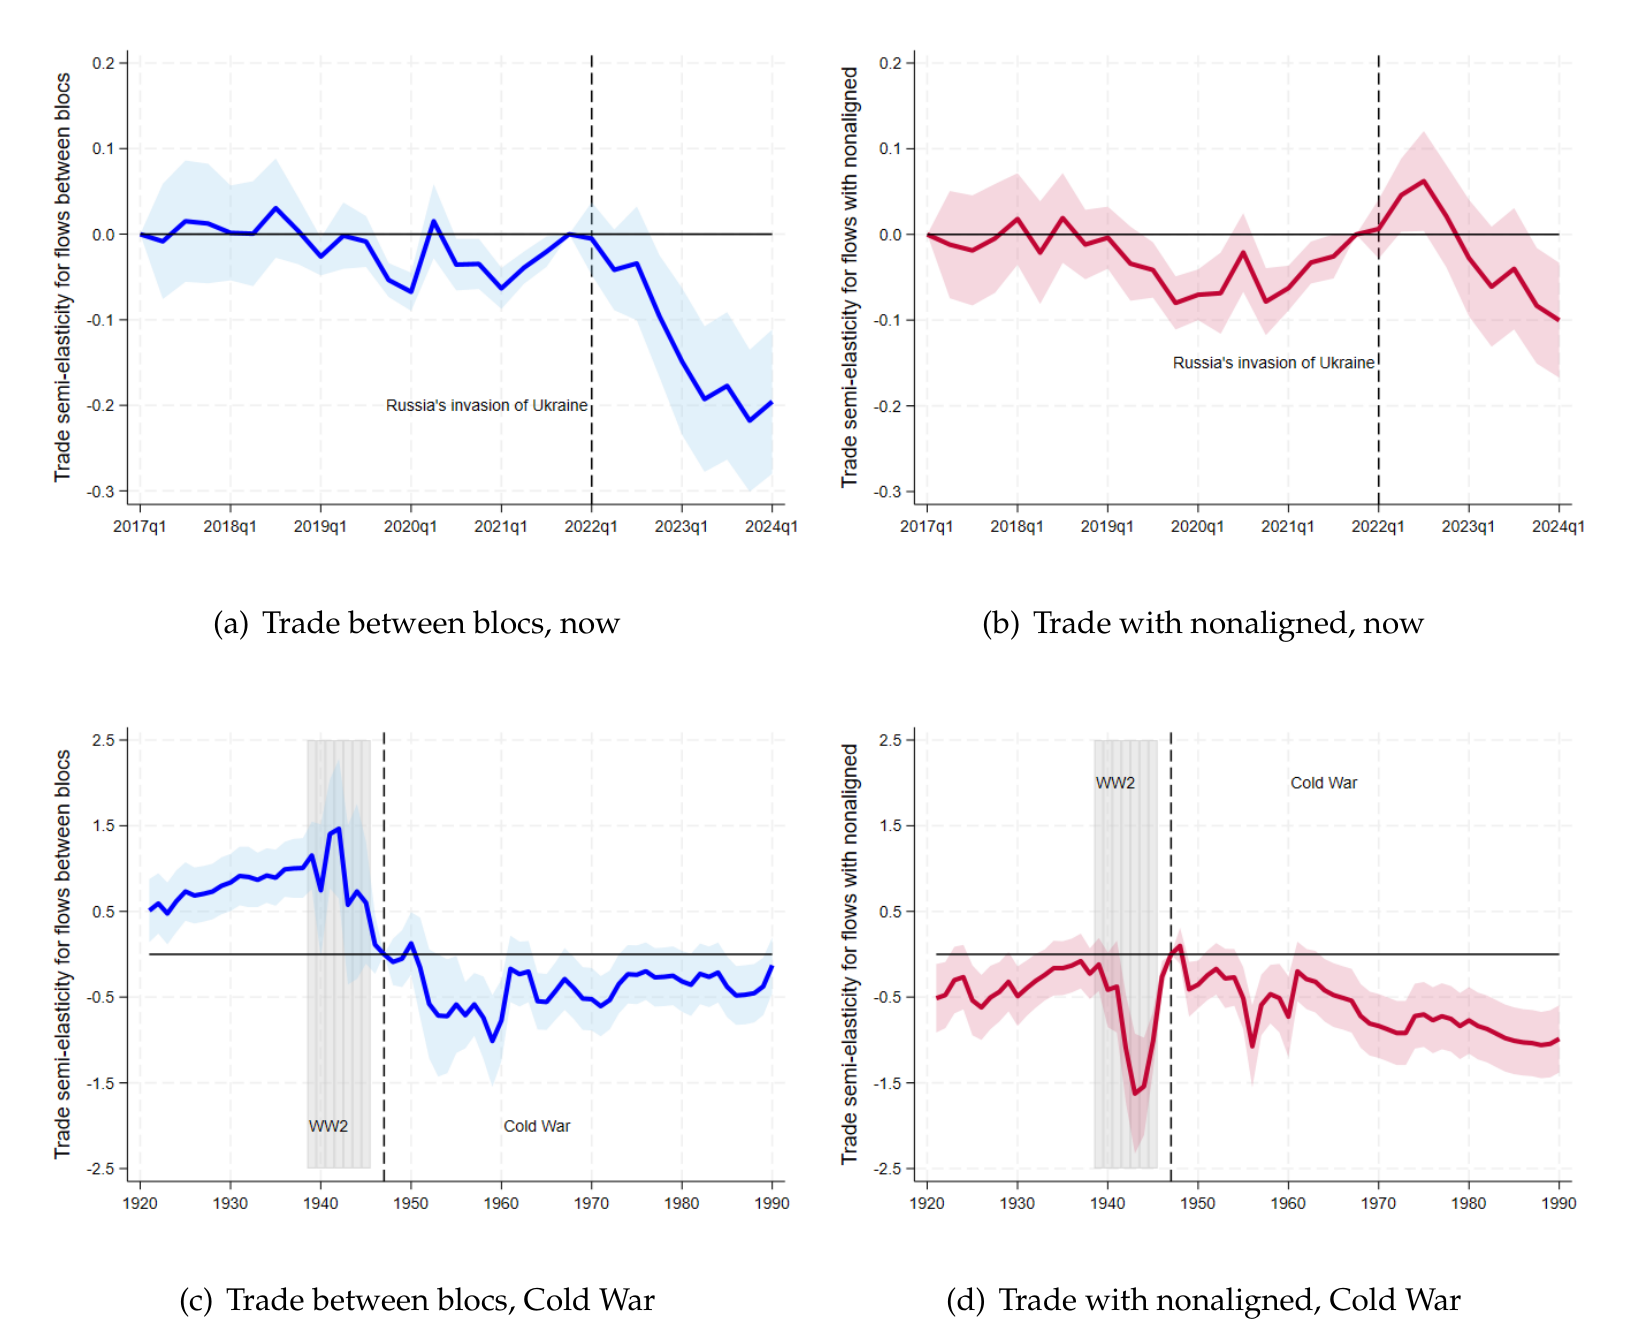
\includegraphics[height=0.9\textheight]{replication_audit/charts_original/FS1.2.png}
  \end{center}
  % \slideclaim{After 2022, cross-bloc trade falls while nonaligned trade is more resilient but recently weakens.}
\end{frame}

\begin{frame}{Connector countries: modern trade and FDI links}
  \begin{center}
    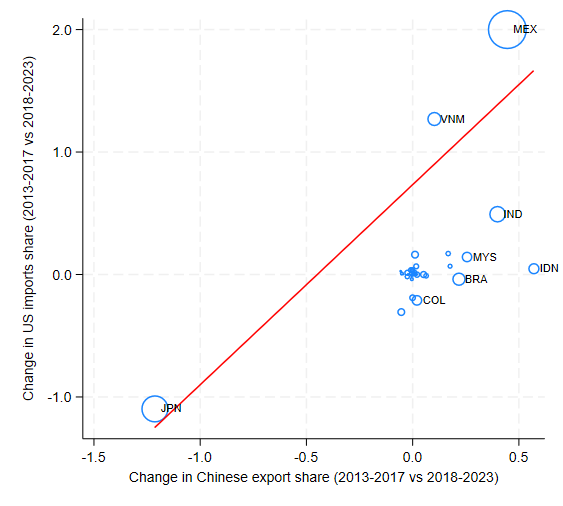
\includegraphics[width=0.46\textwidth]{replication_audit/charts_original/F4A.png}
    \hfill
    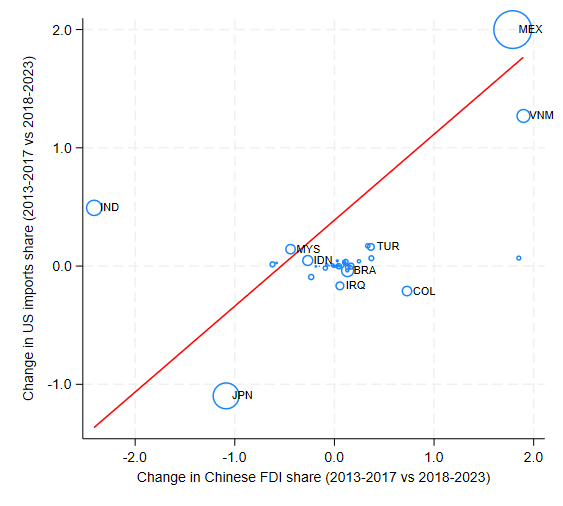
\includegraphics[width=0.46\textwidth]{replication_audit/charts_original/F4C.png}
  \end{center}
  \slideclaim{Panels A and C show a strong and economically large association between stronger Chinese presence in a country and deeper trade links with the United States. A 1 percentage point rise in US import share is associated with a 1.6 percentage point rise in Chinese export share and a 0.7 percentage point rise in Chinese FDI share.}
\end{frame}

\begin{frame}{Connector countries: Cold War contrast}
  \begin{center}
    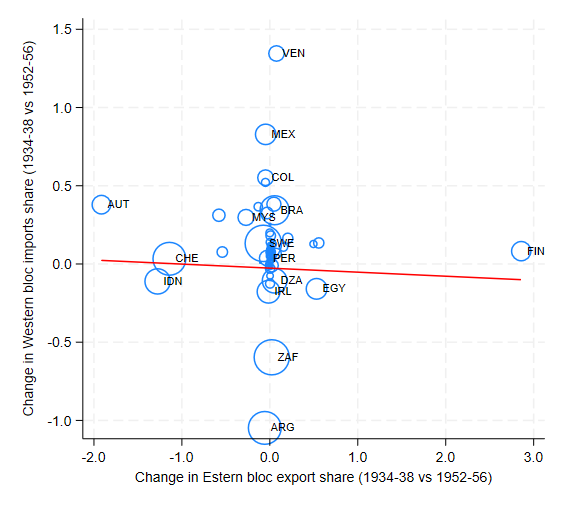
\includegraphics[height=0.60\textheight]{replication_audit/charts_original/F4B.png}
  \end{center}
  \slideclaim{Panel B is the Cold War contrast: Western import share changes and Eastern export share changes are unrelated for nonaligned countries, so they did not operate as connectors between rival blocs.}
\end{frame}

\begin{frame}{Connector Countries}
  \widefig{width=0.95\textwidth}{replication_audit/charts_original/FS1.4.png}
\end{frame}

\begin{frame}{Connector Countries}
  \widefig{width=0.95\textwidth}{replication_audit/charts_original/FS1.6.png}
\end{frame}

\begin{frame}{Connector Countries}
  \widefig{width=0.95\textwidth}{replication_audit/charts_original/FS1.7.png}
\end{frame}

\begin{frame}{Conclusion}
  \begin{itemize}
    \item Geoeconomic fragmentation is visible: trade, FDI, and portfolio positions between blocs have weakened relative to within bloc links.
    \item Fragmentation is not the same as deglobalization. Cold War and current evidence both show that between bloc decoupling can coexist with resilient aggregate trade.
    \item The mechanism has changed. Cold War resilience came mainly from within bloc integration and technology; today, connector countries reroute part of the adjustment.
    \item That creates a policy conundrum. De-risking may lower direct exposure, while connector routes leave underlying dependence partly intact and make supply chains longer, less transparent, and potentially more fragile.
  \end{itemize}
\end{frame}

% \begin{frame}{Economic mechanism}
%   \begin{itemize}
%     \item Direct China US trade falls in politically sensitive sectors.
%     \item Some nonaligned economies gain US market share.
%     \item Those same economies also increase Chinese export exposure or receive more Chinese FDI.
%     \item The policy objective is de-risking, but the equilibrium outcome can be indirect exposure.
%     \item Supply chains may become longer and harder to monitor, rather than simpler and safer.
%   \end{itemize}
%   \slideclaim{The paper's strongest economic insight is that fragmentation can produce rerouting rather than clean decoupling. That weakens the effectiveness of friend shoring as a tool for reducing ultimate exposure.}
% \end{frame}

% \begin{frame}{Empirical design: what the method does well}
%   \begin{tabular}{p{0.30\linewidth}p{0.60\linewidth}}
%     \toprule
%     Design choice                            & Why it is reasonable for this question                                                       \\
%     \midrule
%     PPML gravity                             & Handles zero heavy bilateral flows and keeps the model close to standard trade practice.     \\
%     \midrule
%     Country pair fixed effects               & Remove persistent bilateral frictions such as distance, language, and inherited trade links. \\
%     \midrule
%     Source time and destination time effects & Absorb country specific demand, supply, and policy shocks in each period.                    \\
%     \midrule
%     Multiple outcomes                        & Trade, FDI, and portfolio evidence make the argument broader than a goods market story.      \\
%     \bottomrule
%   \end{tabular}
% \end{frame}

\begin{frame}{Critical assessment}
  \begin{itemize}
    \item UNGA voting based ideal point distance is a sensible bloc measure, but voting proximity is not the same as economic alignment, security ties, technology controls, or firm level supply chain exposure.
    \item Gross trade is an imperfect guide to ultimate exposure. If a connector imports Chinese inputs, does light processing, and exports to the United States, gross flows may overstate diversification away from China.
    \item The portfolio evidence should be read as CPIS evidence, not ultimate risk exposure. As Coppola et al. show, residency based statistics can assign offshore securities to the issuing affiliate rather than the parent country.
    \item The post 2022 window is still short. The estimates may capture an early adjustment phase; the effects could weaken if policy tensions ease, or strengthen if trade controls and investment screening broaden.
  \end{itemize}
\end{frame}

% \begin{frame}{Position in the literature}
% \begin{itemize}
%   \item The paper extends US China trade war evidence by studying global trade, FDI, and portfolio flows jointly.
%   \item It contributes to the geoeconomic fragmentation literature by turning geopolitical distance into a bilateral flow comparison.
%   \item The AEA Papers and Proceedings follow up by the same authors studies production relocation to third countries.
%   \item Aiyar and Ohnsorge's connector country work clarifies the difference between vertical connectors and horizontal connectors.
% \end{itemize}
% \vspace{0.2cm}
% \slideclaim{The paper is not mainly about lower global trade. It is about the political geography of global production and finance.}
% \end{frame}

\begin{frame}{Takeaways}
  \begin{enumerate}
    \item The evidence supports geopolitical sorting, not aggregate deglobalization.
    \item The modern effect is far smaller than the historical Cold War benchmark.
    \item Nonaligned countries are central because they may bridge rival blocs.
    \item Connector countries make policy harder: direct exposure can fall while indirect exposure persists.
    \item The unresolved macro question is welfare: who pays for a longer, more politicized global network?
  \end{enumerate}
  This is not yet a new Cold War, but it is a measurable rewiring of globalization.
\end{frame}

\end{document}
